\section{File and output formats}

\subsection{Infernal CM files}
\label{section:savefiles}

The file \prog{tutorial/Cobalamin.cm} gives an example of an Infernal ASCII
CM save file. An abridged version is shown here, where (\ldots) mark
deletions made for clarity and space:

\begin{tinysreoutput}
INFERNAL1/a [1.1 | April 2012]
NAME     Cobalamin
ACC      RF00174
DESC     Cobalamin riboswitch
STATES   592
NODES    163
CLEN     191
W        381
ALPH     RNA
RF       yes
CONS     yes
MAP      yes
DATE     Mon Apr 23 10:02:42 2012
COM      [1] cmbuild Cobalamin.cm Cobalamin.rfam10p1.seed.sto
COM      [2] cmcalibrate --mpi Cobalamin.cm
PBEGIN   0.05
PEND     0.05
WBETA    1e-07
QDBBETA1 1e-07
QDBBETA2 1e-15
N2OMEGA  1.52588e-05
N3OMEGA  1.52588e-05
ELSELF   -0.08926734
NSEQ     431
EFFN     6.495564
CKSUM    2307274568
NULL     0.000  0.000  0.000  0.000 
GA       39.00
TC       39.00
NC       38.79
EFP7GF   -9.5021 0.71319
ECMLC    0.70182    -9.36743    -0.85775     1600000      470885  0.002548
ECMGC    0.33728   -31.79454   -22.59141     1600000        8915  0.044868
ECMLI    0.67604    -8.08758     0.24666     1600000      335829  0.003573
ECMGI    0.36696   -22.71025   -14.19458     1600000        9103  0.043942
CM
                                             [ ROOT    0 ]      -      - - - - -
     S     0    -1 0     1     4     0     1   381   608  -8.148  -8.355  -0.026  -6.436                 
    IL     1     1 2     1     4    88   135   384   611  -1.686  -2.369  -1.117  -4.855                  0.000  0.000  0.000  0.000 
    IR     2     2 3     2     3    87   134   383   610  -1.442  -0.798  -4.142                          0.000  0.000  0.000  0.000 
                                             [ MATL    1 ]      1      - u - u -
    ML     3     2 3     5     3    88   134   382   609  -9.101  -0.009  -7.755                          0.108 -0.224 -0.313  0.336 
     D     4     2 3     5     3    81   129   379   606  -6.240  -1.550  -0.632                         
    IL     5     5 3     5     3    86   133   382   609  -1.442  -0.798  -4.142                          0.000  0.000  0.000  0.000 
                                             [ MATL    2 ]      2      - u - u -
    ML     6     5 3     8     3    87   133   381   608  -9.104  -0.009  -7.758                          0.219 -0.156 -0.432  0.260 
     D     7     5 3     8     3    80   128   378   605  -6.174  -1.687  -0.566                         
    IL     8     8 3     8     3    85   132   381   608  -1.442  -0.798  -4.142                          0.000  0.000  0.000  0.000 
(...)
                                             [ MATL   97 ]    150      - C - C -
    ML   585   584 3   587     3     1     1    12    31  -9.104  -0.009  -7.758                         -2.793  1.804 -3.077 -2.029 
     D   586   584 3   587     3     0     0    13    32  -6.174  -1.687  -0.566                         
    IL   587   587 3   587     3     1     1    18    36  -1.442  -0.798  -4.142                          0.000  0.000  0.000  0.000 
                                             [ MATL   98 ]    151      - C - C -
    ML   588   587 3   590     2     1     1     1     1       *   0.000                                 -3.019  1.832 -3.344 -2.201 
     D   589   587 3   590     2     0     0     0     0       *   0.000                                 
    IL   590   590 3   590     2     1     1    13    28  -1.823  -0.479                                  0.000  0.000  0.000  0.000 
                                             [ END    99 ]      -      - - - - -
     E   591   590 3    -1     0     0     0     0     0                                                 
//
HMMER3/f [i1.1 | April 2012]
NAME  Cobalamin
ACC   RF00174
DESC  Cobalamin riboswitch
LENG  191
MAXL  565
ALPH  RNA
RF    yes
MM    no
CONS  yes
CS    yes
MAP   yes
DATE  Mon Apr 23 10:02:42 2012
COM   [1] cmbuild ./Cobalamin.cm Cobalamin.rfam10p1.seed.sto
NSEQ  431
EFFN  4.755248
CKSUM 2307274568
STATS LOCAL MSV      -10.2587  0.71319
STATS LOCAL VITERBI  -12.2500  0.71319
STATS LOCAL FORWARD   -3.9252  0.71319
HMM          A        C        G        U   
            m->m     m->i     m->d     i->m     i->i     d->m     d->d
  COMPO   1.37157  1.39386  1.28215  1.51080
          1.38629  1.38629  1.38629  1.38629
          0.02747  4.30141  4.30141  1.46634  0.26236  0.00000        *
      1   1.30044  1.54718  1.61208  1.15433      1 u u - :
          1.38629  1.38629  1.38629  1.38629
          0.02747  4.30141  4.30141  1.46634  0.26236  1.09861  0.40547
      2   1.23217  1.50559  1.68481  1.20072      2 u u - :
          1.38629  1.38629  1.38629  1.38629
          0.02743  4.30301  4.30301  1.46634  0.26236  1.09861  0.40547
(...)
    190   1.36976  1.24867  1.69389  1.29047    440 c c - :
          1.38629  1.38629  1.38629  1.38629
          0.02743  4.30301  4.30301  1.46634  0.26236  1.09861  0.40547
    191   1.40436  1.26828  1.54714  1.34590    441 c c - :
          1.38629  1.38629  1.38629  1.38629
          0.01381  4.28939        *  1.46634  0.26236  0.00000        *
//
\end{tinysreoutput}

An CM file consists of one or more CMs and associated filter
HMMs. Each CM is immediately followed by its filter HMM, this is
mandatory. Each CM starts with a format version identifier (here,
\prog{INFERNAL1/a}) and ends with \prog{//} on a line by itself. Each
HMM also starts with a format version identifier (here,
\prog{HMMER3/f}) and ends with \prog{//} on a line by itself.  The
format version identifier allows backward compatibility as the
Infernal software evolves: it tells the parser this file is from
Infernal's save file format version a.  The closing \prog{//} allows
Infernal to determine when a CM ends and its profile HMM begins, and
allows multiple CM/filter HMM pairs to be concatenated together into a
single file.

The CM format is divided into two regions. The first region contains
textual information and miscalleneous parameters in a roughly
tag-value scheme.  This section ends with a line beginning with the
keyword \prog{CM}. The second region is a tabular, whitespace-limited
format for the main model parameters.

All emission and transition model parameters are stored as log-odds
scores in bits with three digits of precision to the right of the
decimal point, rounded. 
%For example, a probability of $0.25$ is stored
%as $\log_2 0.25 = -1.38629$. 
The special case of a score of infinity, corresponding to an
impossible emission or transition, is stored as '*'.

Spacing is arranged for human readability, but the parser only cares
that fields are separated by at least one space character.

The CM format is described in more detail below, followed by a
description of the HMMER3 HMM format for the CM's mandatory filter HMM
filter.
%The HMM format is similar but is not described in detail here. See the
%HMMER user guide for more information
%(\url{http://hmmer.janelia.org}{http://hmmer.janelia.org}).

\subsubsection{CM header section}

The header section is parsed line by line in a tag/value format. Each
line type is either \textbf{mandatory} or \textbf{optional} as
indicated. 

\begin{sreitems}{QDBBETA1 <f>}

\item [\emprog{INFERNAL1/a}] Unique identifier for the save file format
  version; the \prog{/a} means that this is INFERNAL1 CM file format
  version a. When INFERNAL changes its save file format, the revision
  code advances. This way, parsers may easily remain backwards
  compatible. The remainder of the line after the \prog{INFERNAL1/a} tag
  is free text that is ignored by the parser. INFERNAL currently writes
  its version number and release date in brackets here,
  e.g. \prog{[1.1 | April 2012]} in this
  example. \textbf{Mandatory.}

\item [\emprog{NAME <s>}] Model name; \prog{<s>} is a single word
containing no spaces or tabs. The name is normally picked up from the
\verb+#=GF ID+ line from a Stockholm alignment file.  If this is not
present, the name is created from the name of the alignment file by
removing any file type suffix. For example, an otherwise nameless CM
built from the alignment file \prog{tRNA.sto} would be named
\prog{tRNA}.  \textbf{Mandatory.}

\item [\emprog{ACC <s>}] Accession number; \prog{<s>} is a one-word
accession number. This is picked up from the \verb+#=GF AC+ line in a
Stockholm format alignment. \textbf{Optional.}

\item [\emprog{DESC <s>}] Description line; \prog{<s>} is a one-line
free text description. This is picked up from the \verb+#=GF DE+ line
in a Stockholm alignment file. \textbf{Optional.}

\item [\emprog{STATES <d>}] Number of states; \prog{<d>}, a positive nonzero
integer, is the number of states in the model.
\textbf{Mandatory.}

\item [\emprog{CLEN <d>}] Consensus model length; \prog{<d>}, a positive nonzero
integer, is the number of consensus positions in the model, which
equals the number of MATL nodes plus the number of MATR nodes plus two
times the number of MATP nodes.
\textbf{Mandatory.}

\item [\emprog{W <d>}] Window length; \prog{<d>}, a positive nonzero
integer, is the length in residues of the maximum expected size of a
hit to this model. This is calculated based on the transition
probabilities of the model\footnote{Specifically, \prog{W} is set as
the \emph{dmax} value for the ROOT\_S state (state 0) from the QDB
algorithm using $\beta$ equal to the \prog{WBETA} value
\cite{NawrockiEddy07}.}  \textbf{Mandatory.}

\item [\emprog{ALPH <s>}] Symbol alphabet type. Currently this will
necessarily be \prog{RNA} for RNA sequence analysis models.
The symbol alphabet size $K$ is set to 4 and the 
symbol alphabet to ``ACGU''. \textbf{Mandatory.}

\item [\emprog{RF <s>}] Reference annotation flag; \prog{<s>} is
either \prog{no} or \prog{yes} (case insensitive). If \prog{yes}, the
reference annotation character field(s) for each match state in the
main model (see below) is valid; if \prog{no}, these characters are
ignored.  Reference column annotation is picked up from a Stockholm
alignment file's \verb+#=GC RF+ line. by \prog{cmbuild}. It is
propagated to alignment outputs, and also may optionally be used to
define consensus match columns in CM 
construction. \textbf{Optional}; assumed to be no if not present.

\item [\emprog{CONS <s>}] Consensus residue annotation flag;
  \prog{<s>} is either \prog{no} or \prog{yes} (case insensitive).  If
  \prog{yes}, the consensus residue field(s) for each match state in
  the main model (see below) is valid. If \prog{no}, these characters
  are ignored. Consensus residue annotation is determined when models
  are built. For models of single sequences, the consensus is the same
  as the query sequence. For models of multiple alignments, the
  consensus is the highest scoring residue or basepair for each match
  state. Upper case MATL\_ML and MATR\_MR (single stranded) residues
  indicate that the model emission's score for the consensus residue
  is $\geq$ to 1.0 bit. Upper case MATP\_MP basepairs indicate that
  the model emission's score for the consensus basepair is $\geq$ to
  3.0 bits.

\item [\emprog{MAP <s>}] Map annotation flag; \prog{<s>} is either
\prog{no} or \prog{yes} (case insensitive).  If set to \prog{yes}, the
map annotation field in the main model (see below) is valid; if
\prog{no}, that field will be ignored.  The CM/alignment map
annotates each match state with the index of the alignment column from
which it came. It can be used for quickly mapping any subsequent
CM alignment back to the original multiple alignment, via the model.
\textbf{Optional}; assumed to be no if not present.

\item [\emprog{DATE <s>}] Date the model was constructed; \prog{<s>}
is a free text date string.  This field is only used for logging
purposes.\footnote{Infernal does not use dates for any purpose other than
human-readable annotation, so it is no more prone than you are to Y2K,
Y2038, or any other date-related eschatology.} \textbf{Optional.}

\item [\emprog{COM [<n>] <s>}] Command line log; \prog{<n>} counts
command line numbers, and \prog{<s>} is a one-line command. There may
be more than one \prog{COM} line per save file, each numbered starting
from $n=1$. These lines record every Infernal command that modified the
save file. This helps us reproducibly and automatically log how Rfam
models have been constructed, for example. \textbf{Optional.}

\item [\emprog{PBEGIN <f>}] Local begin probability; The aggregate
probability of a local begin into any internal entry state is
\prog{<f>}. The probability of a local begin into any single internal
entry state is \prog{<f>} divided by the number of internal entry
states in the model. All MATP\_MP, MATL\_ML, MATR\_MR, and BIF\_B
states, except for any in the the second node of the model (first
non-ROOT node), are internal entry states. The local begin probability
does not affect any of the emission/transition parameters in the CM
file, which correspond to the CM in \emph{global} search/alignment
mode, but it does affect the calibration of E-value parameters for
local search by \prog{cmcalibrate}. \prog{cmsearch} and \prog{cmscan}
therefore need to read this probability from the CM file in order to
use the same local begin probabilities used during calibration and
report appropriate E-values. \textbf{Optional}; assumed to be $0.05$
if not present.

\item [\emprog{PEND <f>}] Local end probability; The aggregate
probability of a local end out of any internal exit state is
\prog{<f>}. The probability of a local end out of any single internal
entry state is \prog{<f>} divided by the number of internal exit
states in the model. All MATP\_MP, MATL\_ML, MATR\_MR, BEGL\_S, and
BEGR\_S states, except for any for which the following node is an END
node, are internal exit states. The local end probability
does not affect any of the emission/transition parameters in the CM
file, which correspond to the CM in \emph{global} search/alignment
mode, but it does affect the calibration of E-value parameters for
local search by \prog{cmcalibrate}. \prog{cmsearch} and \prog{cmscan}
therefore need to read this probability from the CM file in order to
use the same local end probabilities used during calibration and
report appropriate E-values. \textbf{Optional}; assumed to be $0.05$
if not present.

\item [\emprog{WBETA <f>}] Tail loss probability for calculating
  window length (W); The QDB algorithm \cite{NawrockiEddy07} was used
  to determine the maximum expected length of a hit (W) using a tail
  loss probability of <f>, W was set as the \emph{dmax} value for the
  ROOT\_S state (state 0). \textbf{Mandatory.}

\item [\emprog{QDBBETA1 <f>}] Tail loss probability for calculating
  the tighter of the two sets of query-dependent bands (QDBs); The QDB
  algorithm \cite{NawrockiEddy07} was used to determine the minimum
  and maximum subsequence lengths allowed to align to the subtree
  rooted at each state of the model, using a tail loss $\beta$
  probability of <f>. These minimum and maximum values for each state
  are included in each state line in the main model section, described
  below.  below. The \prog{<f>} value for \prog{QDBBETA2} will be
  less than or equal to the \prog{<f>} value for \prog{QDBBETA1}.
  \textbf{Mandatory.}

\item [\emprog{QDBBETA2 <f>}] Tail loss probability for calculating
  the looser of the two sets of query-dependent bands (QDBs); The QDB
  algorithm \cite{NawrockiEddy07} was used to determine the minimum
  and maximum subsequence lengths allowed to align to the subtree
  rooted at each state of the model, using a tail loss $\beta$
  probability of <f>. These minimum and maximum values for each state
  are included in each state line in the main model section, described
  below. The \prog{<f>} value for \prog{QDBBETA2} will be less than
  or equal to the \prog{<f>} value for \prog{QDBBETA1}.
  \textbf{Mandatory.}

\item [\emprog{N2OMEGA <f>}] The prior probability for the alternative
  ``null2'' model for biased composition
  sequences. \textbf{Mandatory}; but only relevant in \prog{cmsearch} and
  \prog{cmscan} if the \prog{--null2} option is used.

\item [\emprog{N3OMEGA <f>}] The prior probability for the alternative
  ``null3'' model for biased composition
  sequences. \textbf{Mandatory}; the null3 model is used by default in 
  \prog{cmcalibrate}, \prog{cmsearch} and \prog{cmscan}.

\item [\emprog{NSEQ <d>}] Sequence number; \prog{<d>} is a nonzero
positive integer, the number of sequences that the CM was trained on,
i.e. the number of sequences in the input alignment used to create the
CM in \prog{cmbuild}.  This field is only used for logging
purposes.  \textbf{Optional.}

\item [\emprog{EFFN <f>}] Effective sequence number; \prog{<f>} is a
nonzero positive real, the effective total number of sequences
determined by \prog{cmbuild} during sequence weighting, for combining
observed counts with Dirichlet prior information in parameterizing the
model. This field is only used for logging purposes.
\textbf{Optional.}

\item [\emprog{CKSUM <d>}] Training alignment checksum; \prog{<d>} is
  a nonnegative unsigned 32-bit integer. This number is calculated
  from the training sequence data, and used in conjunction with the
  alignment map information to verify that a given alignment is indeed
  the alignment that the map is for. \textbf{Optional.}

\item [\emprog{NULL <f> <f> <f> <f>}] null model emission scores for
  each alphabet symbol. By default, these are all \prog{0.0} but may
  not be if the \prog{--null} option was used in \prog{cmbuild} to
  define alternative null model scores. Because only RNA CMs can be
  built by \prog{cmbuild} there will be four values on this line, one
  each for ``A'', ``C'', ``G'', and ``U''. \textbf{Mandatory.}

\item [\emprog{GA <f>}] Rfam GA gathering threshold bit score.  The GA
bit score threshold is normally picked up from the \verb+#=GF GA+ line
from a Stockholm alignment file.  GA thresholds are generally
considered to be the reliable curated thresholds defining family
membership; for example, in Rfam, these thresholds define what gets
included in Rfam Full alignments based on searches with Rfam Seed
models. \textbf{Optional.}

\item [\emprog{NC <f>}] Rfam NC noise cutoff bit score.
The NC bit score threshold is normally picked up from the
\verb+#=GF NC+ line from a Stockholm alignment file.  
NC thresholds are generally considered to be the
score of the highest-scoring known false positive found by searches
during preparation of the Rfam database. \textbf{Optional.}

\item [\emprog{TC <f>}] Rfam TC trusted cutoff bit score.
The TC bit score threshold is normally picked up from the
\verb+#=GF TC+ line from a Stockholm alignment file.  
TC thresholds are generally considered to be the score of the lowest
scoring believed true positive that is above all known false positives
found by searches during preparation of the Rfam database.
\textbf{Optional.}

\item [\emprog{EFP7GF <f1> <f2>}] Statistical parameters for filter HMM
  E-value calculations in glocal mode for the Forward algorithm. 
  \prog{<f1>} and \prog{<f2>} are $\tau$ and $\lambda$ for exponential
  tails for glocal Forward filter HMM scores. This line is necessary
  in the CM file section rather than the filter HMM file because
  glocal HMM searches are not normally performed in HMMER3, but are
  part of the HMM filter pipeline in Infernal. \textbf{Mandatory.}

\item [\emprog{ECMLC <f1> <f2> <f3> <d1> <d2> <f4>}] Statistical
  parameters needed for E-value calculations for the CM CYK algorithm
  in local mode. This line, along with the next three, with tags
  \prog{ECMGC}, \prog{ECMLI}, and \prog{ECMGI}, must either all be
  present or none of them must be present. If present, the model is
  considered calibrated for E-value statistics. These lines will not
  be present in a model after it is created by \prog{cmbuild} but will
  be added by the \prog{cmcalibrate} program.  \prog{<f1>} and
  \prog{<f2>} are $\lambda$ and $\tau$, the slope and location
  parameters for exponential tails for local CYK scores. $\lambda$
  values must be positive. The remaining values were computed in
  \prog{cmcalibrate} during model calibration: \prog{<f3>} is a
  different $\tau$ value computed for the full histogram of all hits;
  \prog{<d1>} is the database size in residues; \prog{<d2>} is the
  total number of non-overlapping hits of any score found; \prog{<f4>}
  is the fraction of the high-scoring histogram tail fit to an
  exponential tail. Of these parameters, only \prog{<f1>}, \prog{<f2>}
  and \prog{<d2>} are used, the others are only stored in the CM file
  for record keeping purposes.

\item [\emprog{ECMGC <f1> <f2> <f3> <d1> <d2> <f4>}] Statistical
  parameters analogous to those described above in the \prog{ECMLC}
  line, except that these pertain to CM CYK scores in glocal mode.

\item [\emprog{ECMLI <f1> <f2> <f3> <d1> <d2> <f4>}] Statistical
  parameters analogous to those described above in the \prog{ECMLC}
  line, except that these pertain to CM Inside scores in local mode.

\item [\emprog{ECMGI <f1> <f2> <f3> <d1> <d2> <f4>}] Statistical
  parameters analogous to those described above in the \prog{ECMLC}
  line, except that these pertain to CM Inside scores in glocal mode.

\item [\emprog{CM}] Flags the start of the main model
section. \textbf{Mandatory.}

\end{sreitems}

\subsubsection{CM main model section}

All the remaining fields are \textbf{mandatory}.

The model section consistes of two types of lines: node lines and
state lines. Each node line is immediately followed by one or more
state lines, one each for each state within the node. 

\begin{sreitems}{\textbf{State line}}

\item [\textbf{Node line}] Each node line begins with 45 spaces, and
  includes ten fields. 

  The first field is always a \prog{[} character.

  The second is the node type, one of ROOT, MATP, MATL, MATR, BIF,
  BEGL, BEGR, or END. 

  The next field is the index of the node in the
  model, greater than or equal to 0. Node indices are not always in
  increasing order, e.g. node 200 may come on a line before node 100.

  The fourth field is always a \prog{]} character. 

  The next two fields are the \prog{MAP} annotation for this node. If
  \prog{MAP} was \prog{yes} in the header and the node is a MATP
  (match pair) node, then these fields will both be positive integers,
  representing the alignment column indices for the left and right
  halves of this match pair state, respectively. If \prog{MAP} was
  \prog{yes} and the node is a MATL (match left) node, then the first
  field will be the alignment column for this match state and the
  second field will be '-'. If \prog{MAP} was
  \prog{yes} and the node is a MATR (match right) node, then the first
  field will be '-' and the second field will be the alignment column
  for this match state. If the node is any other type, or if the
  \prog{MAP} was \prog{no} in the header, then both fields will be '-'.

  The next two fields are the \prog{CONS} consensus residue(s) for
  this node. If \prog{CONS} was \prog{yes} in the header and the node
  is a MATP (match pair) node, then these fields will both be
  characters, the consensus residues for the left and right halves of
  this match pair state, respectively. If \prog{CONS} was \prog{yes}
  and the node is a MATL (match left) node, then the first field will
  be the consensus residue for this state and the second field will be
  '-'. If \prog{CONS} was \prog{yes} and the node is a MATR (match
  right) node, then the first field will be '-' and the second field
  will be the consensus residue for this state. If the node is
  any other type, or if the \prog{CONS} was \prog{no} in the header,
  then both fields will be '-'.

  The final two fields are the \prog{RF} annotation for this node.
  this node. If \prog{RF} was \prog{yes} in the header and the node is
  a MATP (match pair) node, then these fields will both be characters,
  the reference annotation character for the left and right halves of
  this match pair state, respectively. If \prog{RF} was \prog{yes} and
  the node is a MATL (match left) node, then the first field will be
  the reference annotation character for this state and the second field
  will be '-'. If \prog{RF} was \prog{yes} and the node is a MATR
  (match right) node, then the first field will be '-' and the second
  field will be the reference annotation character for this state. If
  the node is any other type, or if the \prog{CONS} was \prog{no} in
  the header, then both fields will be '-'.

  Each node line is followed by 1 to 6 state
  lines depending on the node type. ROOT, MATL, and MATR node lines
  are followed by 3 state lines. BIF, BEGL, and END nodes are followed
  by 1 state line. BEGLR node lines have 2 state lines after them, and
  MATP node lines are followed by 6 state lines. 

\item [\textbf{State line}] 
  The number of fields on a state line is variable depending on the
  state type and the number of possible transitions from the
  state. The first field is the state type, either ``MP'', ``ML'',
  ``MR'', ``IL'', ``IR'', ``D'', ``B'', ``S'', or ``E''.

  The next field is the state index, these are in increasing order
  starting with 0 (i.e. lower numbered states always occur earlier in the
  file than higher numbered ones). 

  The next field is the index of the highest numbered ``parent''
  state for the current state, where state $a$ is a parent of state
  $b$ if state $a$ can transition to state $b$.

  The next field is the number of parent states for the current
  state. A set of parent states are always contiguously numbered. For
  example, if state $a$ is the highest numbered parent state of $b$
  and $b$ has 3 parent states, then $a-2$, $a-1$, and $a$ are the
  three parent states of $b$.

  The next field is the index of the lowest numbered ``child'' state
  for the current state, where state $c$ is a child of state $b$ if
  $b$ can transition to state $c$. 

  The next field is the number of child states for the current
  state. A set of child states are always contiguously numbered. For
  example, if state $c$ is the lowest numbered parent state of $b$ and
  $b$ has 3 parent states, then $c$, $c+1$, and $c+2$ are the three
  child states of $b$. As a special case, for ``B'' (bifurcation) states
  this field is the state index of the ``BEGR\_S'' state to which the
  ``B'' state necessarily transitions with probability 1.0.

  The next four fields \prog{<n1>}, \prog{<n2>}, \prog{<n3>}, and
  \prog{<n4>} are query dependent band values for the current
  state. These are integers. \prog{<n1>} is the minimum expected
  subsequence length to align at the subtree rooted at this state
  calculated with the QDB algorithm \cite{NawrockiEddy07} using a
  $\beta$ tail loss probability value given in the header in the
  \prog{QDBBETA2} line. \prog{<n2>} is the same, but calculated with
  $\beta$ equal to the value from the \prog{QDBBETA1} header line. 
  \prog{<n3>} is the maximum expected
  subsequence length to align at the subtree rooted at this state
  calculated with the QDB algorithm \cite{NawrockiEddy07} using a
  $\beta$ tail loss probability value given in the header in the
  \prog{QDBBETA1} line. \prog{<n4>} is the same, but calculated with
  $\beta$ equal to the value from the \prog{QDBBETA2} header line. 
  These values should be in increasing order: $<n1> \leq <n2> \leq
  <n3> \leq <n4>$, although Infernal does not enforce this to be
  true. The QDB values will only be used by \prog{cmsearch} and
  \prog{cmscan} if certain option combinations are used (see the
  manual page for those programs); by default they are not used.

  After the four QDB values, the next set of fields are log-odds bit
  scores for possible transitions out of this state to all child
  states of the current states. The number of child states is given
  earlier on the line as the sixth field. It varies depending on the
  state type and the node type of the \emph{next} node in the model.
  For a list of all possible sets of transitions for each possible
  state type/next node combination see Table 1 of
  \cite{NawrockiEddy07}. As a special case, ``B'' (bifurcation) states
  have zero transition score fields, they necessarily transition to
  their child ``BEGL\_S'' and ``BEGR\_S'' states with a probability of
  $1.0$ (score of $0$ bits).

  After the transition scores are the emission scores. 
  ``MP'' state lines have 16 emission log-odds bit scores. All other
  types of emitting states (``ML'', ``MR'', ``IL'', ``IR'') will have
  four emission scores. All other types of states will have no
  emission scores. For ``MP'' states, the sixteen scores are for the
  sixteen possible non-degenerate RNA basepairs: ``AA'', ``AC'',
  ``AG'', ``AU'', ``CA'', ``CC'', ``CG'', ``CU'', ``GA'', ``GC'',
  ``GG'', ``GU'', ``UA'', ``UC'', ``UG'', ``UU'', in that order. 
  For the other emitting states the four scores are for ``A'', ``C'',
  ``G'', and ``U'', in that order.
\end{sreitems}

  Finally, the last line of the format is the ``//'' record separator.
  After the CM comes its associated filter HMM in HMMER3 format,
  described below.

\subsubsection{HMMER3 filter HMM format}

As with the CM, the HMM format is divided into two regions. The first
region contains textual information and miscalleneous parameters in a
roughly tag-value scheme.  This section ends with a line beginning
with the keyword \prog{HMM}. The second region is a tabular,
whitespace-limited format for the main model parameters.

All HMM probability parameters are all stored as negative natural log
probabilities with five digits of precision to the right of the
decimal point, rounded. For example, a probability of $0.25$ is stored
as $-\log 0.25 = 1.38629$. The special case of a zero probability is
stored as '*'.

Spacing is arranged for human readability, but the parser only cares
that fields are separated by at least one space character.

A more detailed description of the format follows.

\subsubsection{HMM header section}

The header section is parsed line by line in a tag/value format. Each
line type is either \textbf{mandatory} or \textbf{optional} as
indicated. 

\begin{sreitems}{\emprog{STATS <s1> <s2> <f>}}

\item [\emprog{HMMER3/f}] Unique identifier for the save file format
  version; the \prog{/b} means that this is HMMER3 HMM file format
  version b. When HMMER3 changes its save file format, the revision
  code advances. This way, parsers may easily remain backwards
  compatible. The remainder of the line after the \prog{HMMER3/b} tag
  is free text that is ignored by the parser. HMMER currently writes
  its version number and release date in brackets here,
  e.g. \prog{[3.0b2 | June 2009]} in this
  example. \textbf{Mandatory.}

\item [\emprog{NAME <s>}] Model name; \prog{<s>} is a single word
containing no spaces or tabs. The name is normally picked up from the
\verb+#=GF ID+ line from a Stockholm alignment file.  If this is not
present, the name is created from the name of the alignment file by
removing any file type suffix. For example, an otherwise nameless HMM
built from the alignment file \prog{rrm.slx} would be named
\prog{rrm}.  \textbf{Mandatory.}

\item [\emprog{ACC <s>}] Accession number; \prog{<s>} is a one-word
accession number. This is picked up from the \verb+#=GF AC+ line in a
Stockholm format alignment. \textbf{Optional.}

\item [\emprog{DESC <s>}] Description line; \prog{<s>} is a one-line
free text description. This is picked up from the \verb+#=GF DE+ line
in a Stockholm alignment file. \textbf{Optional.}

\item [\emprog{LENG <d>}] Model length; \prog{<d>}, a positive nonzero
integer, is the number of match states in the model.
\textbf{Mandatory.}

\item [\emprog{ALPH <s>}] Symbol alphabet type. For biosequence
analysis models, \prog{<s>} is \prog{amino}, \prog{DNA}, or \prog{RNA}
(case insensitive). There are also other accepted alphabets for
purposes beyond biosequence analysis, including \prog{coins},
\prog{dice}, and \prog{custom}. This determines the symbol alphabet
and the size of the symbol emission probability distributions.  If
\prog{amino}, the alphabet size $K$ is set to 20 and the symbol
alphabet to ``ACDEFGHIKLMNPQRSTVWY'' (alphabetic order); if
\prog{DNA}, the alphabet size $K$ is set to 4 and the symbol alphabet
to ``ACGT''; if \prog{RNA}, the alphabet size $K$ is set to 4 and the
symbol alphabet to ``ACGU''. \textbf{Mandatory.}

\item [\emprog{RF <s>}] Reference annotation flag; \prog{<s>} is
either \prog{no} or \prog{yes} (case insensitive). If \prog{yes}, the
reference annotation character field for each match state in the main
model (see below) is valid; if \prog{no}, these characters are
ignored.  Reference column annotation is picked up from a Stockholm
alignment file's \verb+#=GC RF+ line. It is propagated to alignment
outputs, and also may optionally be used to define consensus match
columns in profile HMM construction. \textbf{Optional}; assumed to be
no if not present.

\item [\emprog{CONS <s>}] Consensus residue annotation flag;
  \prog{<s>} is either \prog{no} or \prog{yes} (case insensitive).  If
  \prog{yes}, the consensus residue field for each match state in the
  main model (see below) is valid. If \prog{no}, these characters are
  ignored. Consensus residue annotation is determined when models are
  built. For models of single sequences, the consensus is the same as
  the query sequence. For models of multiple alignments, the consensus
  is the maximum likelihood residue at each position. Upper case
  indicates that the model's emission probability for the consensus
  residue is $\geq$ an arbitrary threshold (0.5 for protein models,
  0.9 for DNA/RNA models).

\item [\emprog{CS <s>}] Consensus structure annotation flag;
\prog{<s>} is either \prog{no} or \prog{yes} (case insensitive). If
\prog{yes}, the consensus structure character field for each match
state in the main model (see below) is valid; if \prog{no} these
characters are ignored. Consensus structure annotation is picked up
from a Stockholm file's \verb+#=GC SS_cons+ line, and propagated to
alignment displays.  \textbf{Optional}; assumed to be no if not
present.

\item [\emprog{MAP <s>}] Map annotation flag; \prog{<s>} is either
\prog{no} or \prog{yes} (case insensitive).  If set to \prog{yes}, the
map annotation field in the main model (see below) is valid; if
\prog{no}, that field will be ignored.  The HMM/alignment map
annotates each match state with the index of the alignment column from
which it came. It can be used for quickly mapping any subsequent
HMM alignment back to the original multiple alignment, via the model.
\textbf{Optional}; assumed to be no if not present.

\item [\emprog{DATE <s>}] Date the model was constructed; \prog{<s>}
is a free text date string.  This field is only used for logging
purposes.\footnote{HMMER does not use dates for any purpose other than
human-readable annotation, so it is no more prone than you are to Y2K,
Y2038, or any other date-related eschatology.} \textbf{Optional.}

\item [\emprog{COM [<n>] <s>}] Command line log; \prog{<n>} counts
command line numbers, and \prog{<s>} is a one-line command. There may
be more than one \prog{COM} line per save file, each numbered starting
from $n=1$. These lines record every HMMER command that modified the
save file. This helps us reproducibly and automatically log how Pfam
models have been constructed, for example. \textbf{Optional.}

\item [\emprog{NSEQ  <d>}] Sequence number; \prog{<d>} is a nonzero
positive integer, the number of sequences that the HMM was trained on.
This field is only used for logging purposes.
\textbf{Optional.}

\item [\emprog{EFFN <f>}] Effective sequence number; \prog{<f>} is a
nonzero positive real, the effective total number of sequences
determined by \prog{hmmbuild} during sequence weighting, for combining
observed counts with Dirichlet prior information in parameterizing the
model. This field is only used for logging purposes.
\textbf{Optional.}

\item [\emprog{CKSUM <d>}] Training alignment checksum; \prog{<d>} is
  a nonnegative unsigned 32-bit integer. This number is calculated
  from the training sequence data, and used in conjunction with the
  alignment map information to verify that a given alignment is indeed
  the alignment that the map is for. \textbf{Optional.}

\item [\emprog{GA    <f> <f>}] Pfam gathering thresholds GA1 and GA2.
See Pfam documentation of GA lines. \textbf{Optional.}

\item [\emprog{TC <f> <f>}] Pfam trusted cutoffs TC1 and TC2.  See
Pfam documentation of TC lines. \textbf{Optional.}

\item [\emprog{NC <f> <f>}] Pfam noise cutoffs NC1 and NC2.  See Pfam
documentation of NC lines. \textbf{Optional.}

\item [\emprog{STATS <s1> <s2> <f1> <f2>}] Statistical parameters
  needed for E-value calculations. \prog{<s1>} is the model's
  alignment mode configuration: currently only \prog{LOCAL} is
  recognized. \prog{<s2>} is the name of the score distribution:
  currently \prog{MSV}, \prog{VITERBI}, and \prog{FORWARD} are
  recognized.  \prog{<f1>} and \prog{<f2>} are two real-valued
  parameters controlling location and slope of each distribution,
  respectively; $\mu$ and $\lambda$ for Gumbel distributions for MSV
  and Viterbi scores, and $\tau$ and $\lambda$ for exponential tails
  for Forward scores.  $\lambda$ values must be positive.  All three
  lines or none of them must be present: when all three are present,
  the model is considered to be calibrated for E-value
  statistics. \textbf{Optional.}

\item [\emprog{HMM }] Flags the start of the main model
section. Solely for human readability of the tabular model data, the
symbol alphabet is shown on the \prog{HMM} line, aligned to the fields
of the match and insert symbol emission distributions in the main
model below. The next line is also for human readability, providing
column headers for the state transition probability fields in the main
model section that follows. Though unparsed after the \prog{HMM} tag,
the presence of two header lines is \textbf{mandatory:} the parser
always skips the line after the \prog{HMM} tag line.

\item [\emprog{COMPO <f>*K}] The first line in the main model section
may be an optional line starting with \emprog{COMPO}: these are the
model's overall average match state emission probabilities, which are
used as a background residue composition in the ``filter null''
model. The $K$ fields on this line are log probabilities for each
residue in the appropriate biosequence alphabet's
order. \textbf{Optional.}

\end{sreitems}

\subsubsection{HMM main model section}

All the remaining fields are \textbf{mandatory}.

The first two lines in the main model section are
atypical.\footnote{That is, the first two lines after the optional
  COMPO line. Don't be confused by the presence of an optional COMPO
  line here. The COMPO line is placed in the model section, below the
  residue column headers, because it's an array of numbers much like
  residue scores, but it's not really part of the model.}  They
contain information for the core model's BEGIN node. This is stored as
model node 0, and match state 0 is treated as the BEGIN state.  The
begin state is mute, so there are no match emission probabilities. The
first line is the insert 0 emissions. The second line contains the
transitions from the begin state and insert state 0.  These seven
numbers are: $B \rightarrow M_1$, $B \rightarrow I_0$, $B \rightarrow
D_1$; $I_0 \rightarrow M_1$, $I_0 \rightarrow I_0$; then a 0.0 and a
'*', because by convention, nonexistent transitions from the
nonexistent delete state 0 are set to $\log 1 = 0$ and $\log 0 =
-\infty = $ `*'.

The remainder of the model has three lines per node, for $M$ nodes
(where $M$ is the number of match states, as given by the \prog{LENG}
line). These three lines are ($K$ is the alphabet size in residues):

\begin{sreitems}{\textbf{State transition line}}

\item [\textbf{Match emission line}] The first field is the node
number ($1 \ldots M$).  The parser verifies this number as a
consistency check (it expects the nodes to come in order). The next
$K$ numbers for match emissions, one per symbol, in alphabetic order.

The next field is the \prog{MAP} annotation for this node.  If
\prog{MAP} was \prog{yes} in the header, then this is an integer,
representing the alignment column index for this match state
(1..alen); otherwise, this field is `-'.

The next field is the \prog{CONS} consensus residue for this node.  If
\prog{CONS} was \prog{yes} in the header, then this is a single
character, representing the consensus residue annotation for this
match state; otherwise, this field is `-'.

The next field is the \prog{RF} annotation for this node.  If
\prog{RF} was \prog{yes} in the header, then this is a single
character, representing the reference annotation for this match state;
otherwise, this field is `-'.

The next field is the \prog{CS} annotation for this node.  If
\prog{CS} was \prog{yes}, then this is a single character,
representing the consensus structure at this match state; otherwise
this field is `-'.

\item [\textbf{Insert emission line}] The $K$ fields on this line are
the insert emission scores, one per symbol, in alphabetic order.

\item [\textbf{State transition line}] The seven fields on this line
are the transitions for node $k$, in the order shown by the transition
header line: $M_k \rightarrow M_{k+1}, I_{k}, D_{k+1}$; $ I_k
\rightarrow M_{k+1}, I_k$; $D_{k} \rightarrow M_{k+1}, D_{k+1}$.

For transitions from the final node $M$, match state $M+1$ is
interpreted as the END state $E$, and there is no delete state $M+1$;
therefore the final $M_k \rightarrow D_{k+1}$ and $D_k \rightarrow
D_{k+1}$ transitions are always * (zero probability), and the final
$D_k \rightarrow M_{k+1}$ transition is always 0.0 (probability 1.0).
\end{sreitems}

Finally, the last line of the format is the ``//'' record separator.

\subsection{RNA secondary structures: WUSS notation}
\label{section:wuss}

Infernal annotates RNA secondary structures using a linear
string representation called ``WUSS notation'' (Washington University
Secondary Structure notation).

The symbology is extended from the common bracket notation for RNA
secondary structures, where open- and close-bracket symbols (or
parentheses) are used to annotate base pairing partners: for example,
\verb+((((...))))+ indicates a four-base stem with a three-base loop.
Bracket notation is difficult for humans to interpret, for anything
much larger than a simple stem-loop. WUSS notation makes it somewhat
easier to interpret the annotation for larger structures.

The following figure shows an example with the key elements of WUSS
notation.  At the top left is an example RNA structure. At the top
right is the same structure, with different RNA structural elements
marked. Below both structure pictures : the WUSS notation string for
the structure.

\begin{center}
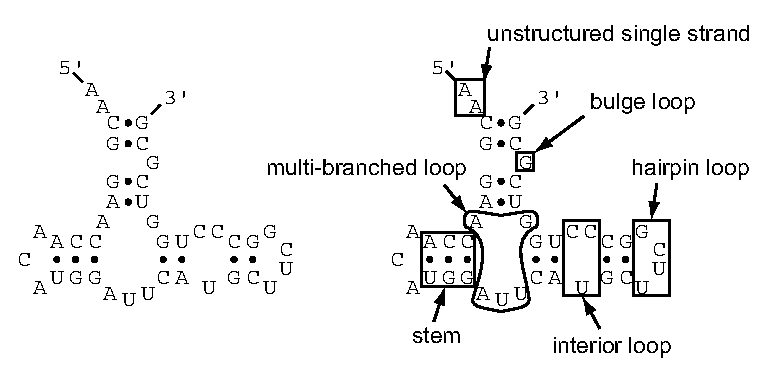
\includegraphics[scale=0.8]{Figures/rna_elements}
\end{center}
\begin{center}
\begin{BVerbatim}
  ::((((,<<<___>>>,,,<<-<<____>>-->>,))-))
  AACGGAACCAACAUGGAUUCAUGCUUCGGCCCUGGUCGCG
\end{BVerbatim}
\end{center}

\subsubsection{Full (output) WUSS notation}

In detail, symbols used by WUSS notation in \emph{output} structure
annotation strings are as follows:

\begin{sreitems}{\textbf{Bulge, interior loops}}
\item[\textbf{Base pairs}]
  Base pairs are annotated by nested matching pairs of symbols
  \verb+<>+, \verb+()+, \verb+[]+, or \verb+{}+.
  The different symbols indicate the ``depth'' of the
  helix in the RNA structure as follows:
  \verb+<>+ are used for simple terminal stems; 
  \verb+()+ are used for ``internal'' helices enclosing a multifurcation of
  all terminal stems; \verb+[]+ are used for internal helices 
  enclosing a multifurcation that includes at least one annotated
  \verb+()+ stem already; and \verb+{}+ are used for all internal
  helices enclosing deeper multifurcations.
   
\item[\textbf{Hairpin loops}]
  Hairpin loop residues are indicated by underscores, \verb+_+.
  Simple stem loops stand out as, e.g.\ \verb+<<<<____>>>>+.

\item[\textbf{Bulge, interior loops}]
  Bulge and interior loop residues are indicated by dashes, \verb+-+.
  
\item[\textbf{Multifurcation loops}]
  Multifurcation loop residues are indicated by commas, \verb+,+.
  The mnemonic is ``stem 1, stem2'', e.g.\ \verb+<<<___>>>,,<<<___>>>+.

\item[\textbf{External residues}]
  Unstructured single stranded residues completely outside the
  structure (unenclosed by any base pairs) are annotated by
  colons, \verb+:+.

\item[\textbf{Insertions}]
  Insertions relative to a known structure are indicated by periods,
  \verb+.+. Regions where local structural alignment was invoked,
  leaving regions of both target and query sequence unaligned,
  are indicated by tildes, \verb+~+. These symbols only appear in
  alignments of a known (query) structure annotation to a target
  sequence of unknown structure.

\item[\textbf{Pseudoknots}]
  WUSS notation allows pseudoknots to be annotated as pairs of
  upper case/lower case letters: for example,
  \verb+<<<<_AAAA____>>>>aaaa+ annotates a simple pseudoknot;
  additional pseudoknotted stems could be annotated by \verb+Bb+,
  \verb+Cc+, etc. \software{infernal} cannot handle pseudoknots, however;
  pseudoknot notation never appears in \software{infernal} output; it
  is accepted in input files, but ignored.
\end{sreitems}

An example of WUSS notation for a complicated structure
(\emph{E. coli} RNase P) is shown in Figure~\ref{fig:RNaseP}.  An
example of WUSS notation for a local \software{infernal} alignment of
\emph{B. subtilis} RNase P to \emph{E. coli} RNase P, illustrating the
use of local alignment annotation symbols, is in
Figure~\ref{fig:bsu-alignment}.

\begin{figure}[tp]
\begin{center}
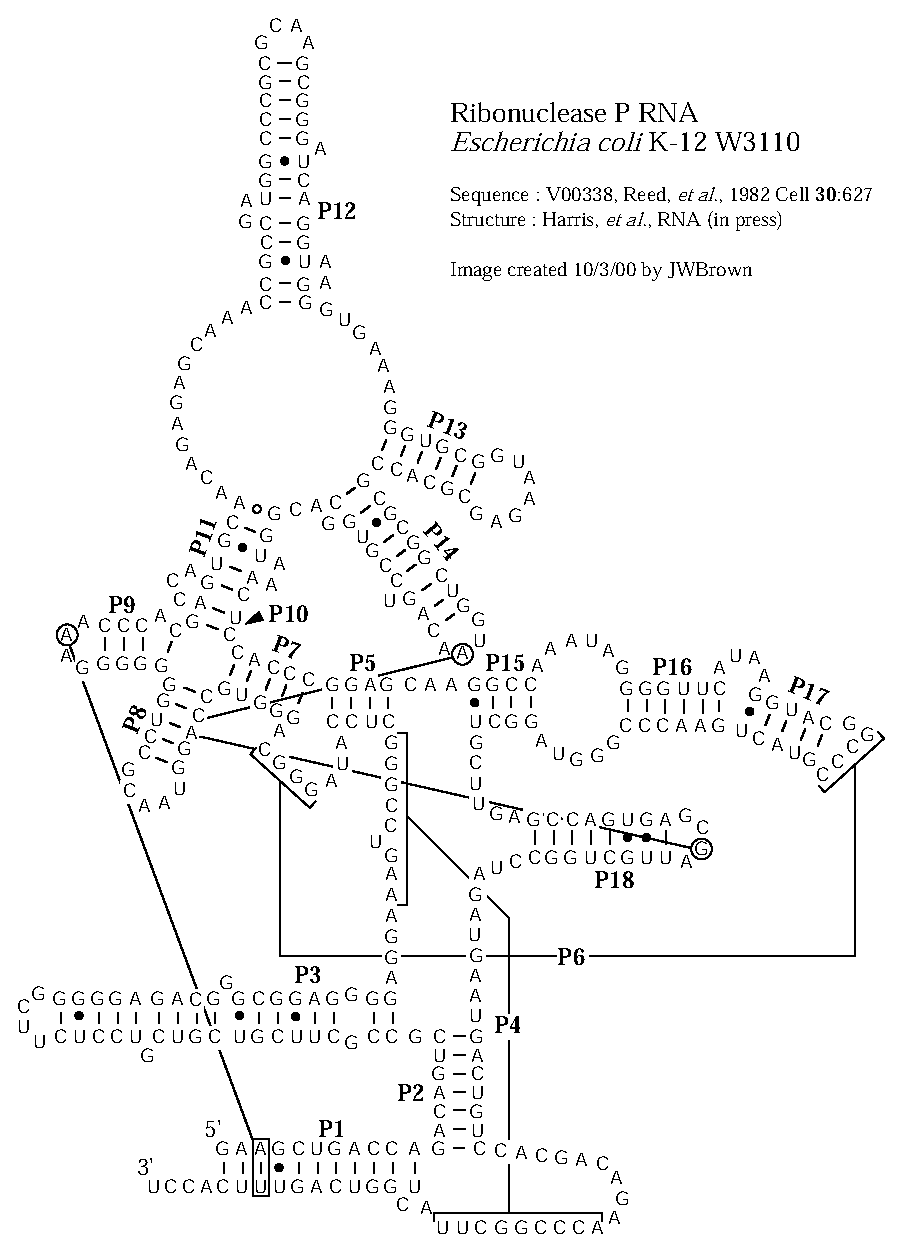
\includegraphics[scale=0.6]{Figures/rnaseP-ecoli}
\end{center}        
\begin{center}
{\scriptsize
\begin{BVerbatim}
           {{{{{{{{{{{{{{{{{{,<<<<<<<<<<<<<-<<<<<____>>>>>>>>>->>>>>>>>
         1 GAAGCUGACCAGACAGUCGCCGCUUCGUCGUCGUCCUCUUCGGGGGAGACGGGCGGAGGG 60      

           >,,,,,,,,,,,,,[[[[--------[[[[[<<<<<_____>>>>><<<<____>>>->(
        61 GAGGAAAGUCCGGGCUCCAUAGGGCAGGGUGCCAGGUAACGCCUGGGGGGGAAACCCACG 120     

           (---(((((,,,,,,,,,,,,<<<<<--<<<<<<<<____>>>>>->>>>>>-->>,,,,
       121 ACCAGUGCAACAGAGAGCAAACCGCCGAUGGCCCGCGCAAGCGGGAUCAGGUAAGGGUGA 180     

           ,,,<<<<<<_______>>>>>><<<<<<<<<____>>>->>>>>->,,)))--))))]]]
       181 AAGGGUGCGGUAAGAGCGCACCGCGCGGCUGGUAACAGUCCGUGGCACGGUAAACUCCAC 240     

           ]]]]]],,,<<<<------<<<<<<----<<<<<_____>>>>>>>>>>>----->>>>,
       241 CCGGAGCAAGGCCAAAUAGGGGUUCAUAAGGUACGGCCCGUACUGAACCCGGGUAGGCUG 300     

           ,,,,,<<<<<<<<____>>>>>>>>,,,,,,,,,,}}}}}}}------------------
       301 CUUGAGCCAGUGAGCGAUUGCUGGCCUAGAUGAAUGACUGUCCACGACAGAACCCGGCUU 360     

           -}-}}}}}}}}}}::::
       361 AUCGGUCAGUUUCACCU 377     
\end{BVerbatim} 
}
\end{center}
\caption{\small \textbf{Example of WUSS notation.} Top: Secondary
structure of \emph{E. coli} RNase P, from Jim Brown's RNase P database
\cite{Brown99}. Bottom: WUSS notation for the same structure,
annotating the \emph{E. coli} RNase P sequence. The P4 and P6
pseudoknots are not annotated in this example.}
\label{fig:RNaseP}
\end{figure}

\begin{figure}[tp]
\begin{center}
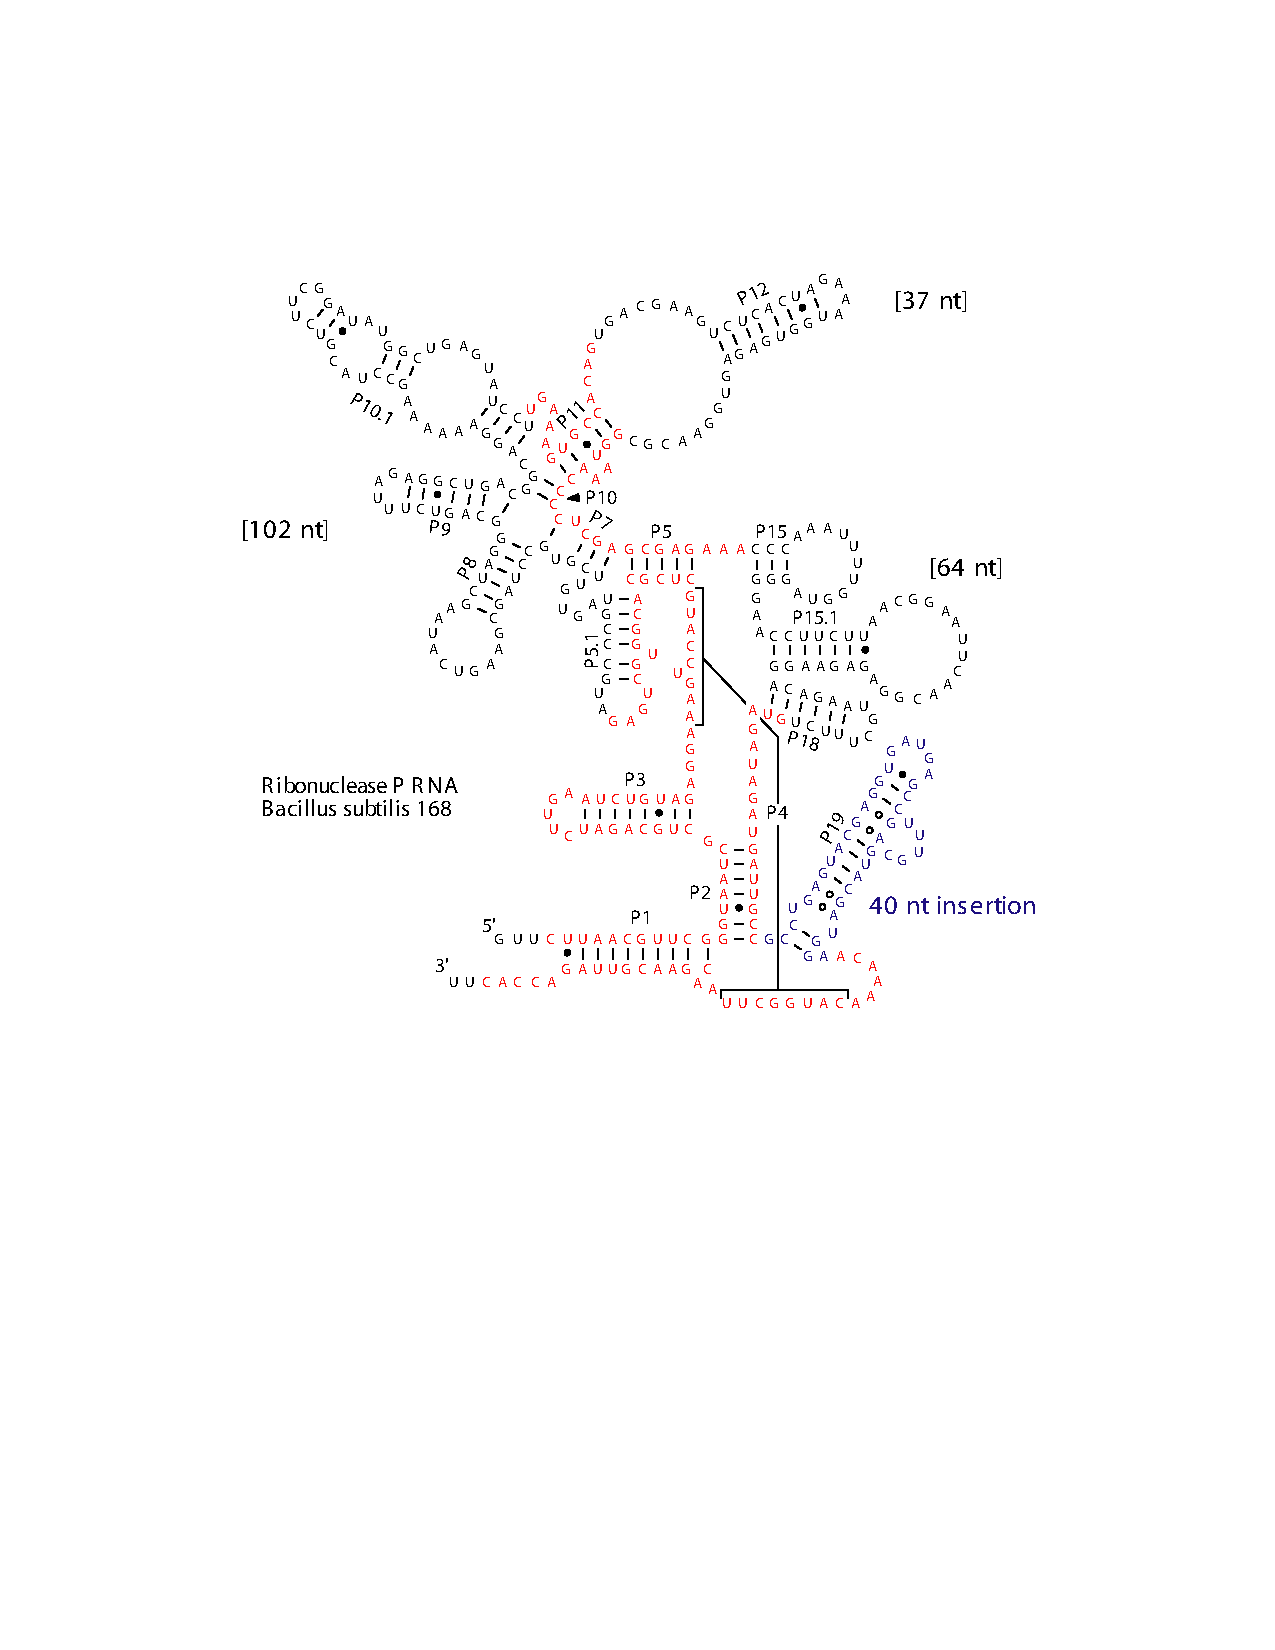
\includegraphics[scale=0.6]{Figures/rnaseP-bsu-alignment}
\end{center}
\begin{center}
{\scriptsize
\begin{BVerbatim}
hit 0   :      4    399    52.56 bits
           {{{{{{{{{{{{{{{{{{,<<<<<<<<<<<<<-<<<<<____>>>>>>>>>->>>>>>>>
         1 ggAGuggGgcaGgCaguCGCugcuucggccuuGuucaguuaacugaaaaggAccgaagga 60      
           +: :::G::C:GG:A:UCGCU+C::::            U+            ::::G+A
         4 CUUAACGUUCGGGUAAUCGCUGCAGAUC-----------UUG----------AAUCUGUA 42      

           >,,,,,,,,,,,,,[[[.[--------[[[[[~~~~~~~((---(((((,,,,~~~~~~)
        61 GAGGAAAGUCCGGGCUC.CACAGGGCAgGGUG*[ 29]*GGAAAGUGCCACAG*[96]*G 229     
           GAGGAAAGUCC  GCUC C  A GG   :G G       :GAAAGUGCCACAG      G
        43 GAGGAAAGUCCAUGCUCgC--ACGGUGCUGAG*[102]*UGAAAGUGCCACAG*[37]*G 226     

           ))--))))]]]]]].]]],,,~~~~~~,,,,,,,,,,}}}}}}}--..............
       230 GUAAACCCCACCcG.GAGCAA*[77]*CuAGAUGAAUGacuGcCCA.............. 344     
           GUAAACC:C C: G GAG AA       UAGAU++AUGA:U:CC                
       227 GUAAACCCCUCGAGcGAGAAA*[64]*GUAGAUAGAUGAUUGCC--gccugaguacgagg 342     

           ..........................-----------------}-}}}}}}}}}}::::
       345 ..........................CGACAGAACCCGGCUUAuagcCccaCUccucuu 377     
                                       ACA AAC  GGCUUA:AG::C::: :+ C  
       343 ugaugagccguuugcaguacgaugga--ACAAAACAUGGCUUACAGAACGUUAGACCAC 399     
\end{BVerbatim}
}
\end{center}
\caption{\small \textbf{Local alignment annotation example.} Top:
Secondary
structure of \emph{B. subtilis} RNase P, from Jim Brown's RNase P
database \cite{Brown99}. Residues in red are those that \software{infernal} aligns
to a CM of \emph{E. coli} type RNase P's. The local structural
alignment is in four pieces; three regions of the
structure (102, 37, and 64 nt long) are skipped over. One additional
stem is treated as a 40 nt insertion. Bottom: the \software{infernal}
output, showing the \emph{E. coli} query structure aligned to the
\emph{B. subtilis} sequence.}
\label{fig:bsu-alignment}
\end{figure}

\subsubsection{Shorthand (input) WUSS notation}

While WUSS notation makes it easier to visually interpret
\software{infernal} \emph{output} structural annotation, it would be
painful to be required to \emph{input} all structures in full WUSS
notation. Therefore when \software{infernal} reads input secondary
structure annotation, it uses simpler rules:

\begin{sreitems}{\textbf{Single stranded residues}}
\item [\textbf{Base pairs}]
  Any matching nested pair of \verb+()+, \verb+()+, \verb+[]+, \verb+{}+
  symbols indicates a base pair; the exact choice of symbol has no
  meaning, so long as the left and right partners match up.

\item [\textbf{Single stranded residues}]
  All other symbols \verb+_-,:.~+ 
  indicate single stranded residues.
  The choice of symbol has no special meaning.
  Annotated pseudoknots (nested matched pairs of upper/lower case
  alphabetic characters) are also interpreted as single
  stranded residue in \software{infernal} input.
\end{sreitems}

Thus, for instance, \verb+<<<<....>>>>+ and \verb+((((____))))+ and
\verb+<(<(._._)>)>+ all indicate a four base stem with a four base
loop (the last example is legal but weird). 

Remember that the key property of canonical (nonpseudoknotted) RNA
secondary structure is that the pairs are \emph{nested}.
\verb+((<<....))>>+ is not a legal annotation string: the pair symbols
don't match up properly. \software{infernal} will reject such an
annotation and report an input format error, suspecting a problem with
your annotation.  If you want to annotate pseudoknots, WUSS notation
allows alphabetic symbols Aa, Bb, etc.\, see above; but remember that
\software{infernal} ignores pseudoknotted stems and treats them as
single stranded residues.

Because many other RNA secondary structure analysis programs use a
simple bracket notation for annotating structure,
\software{infernal}'s ability to input this format makes it easier to
use data generated by other RNA software packages. Conversely,
converting \software{infernal} output WUSS notation to simple bracket
notation is a matter of a simple Perl or sed script, substituting the
symbols appropriately.

\subsection{Stockholm, the recommended multiple sequence alignment format}
\label{section:stockholm}

The Rfam and Pfam Consortiums have developed a multiple sequence
alignment format called ``Stockholm format'' that allows rich and
extensible annotation. 

Crucially for Infernal, Stockholm alignments support the annotation of 
a consensus secondary structure, which is why \prog{cmbuild} requires
its input alignment files to be in Stockholm format. Here is a minimal
Stockholm file with consensus secondary structure annotation in
shorthand WUSS notation (described above in
section~\ref{section:wuss}).

\begin{sreoutput}
# STOCKHOLM 1.0

seq1           ACCGUC...GCAA...GG
seq2           ACCGUC...GCAA...GG
seq3           .CCUUCGUCGGAUGACGA
#=GC SS_cons   ...<<<..........>>

seq1           CGAUAC
seq2           CG..AC
seq3           ACAUCC
#=GC SS_cons   >.....
//
\end{sreoutput}

The first line in the file must be \verb+# STOCKHOLM 1.x+, where
\verb+x+ is a minor version number for the format specification
(and which currently has no effect on my parsers). This line allows a
parser to instantly identify the file format.

In the alignment, each line contains a name, followed by the aligned
sequence. A dash, period, underscore, or tilde (but not whitespace)
denotes a gap. If the alignment is too long to fit on one line, the
alignment may be split into multiple blocks, with blocks separated by
blank lines, as this example is. The number of sequences, their order,
and their names must be the same in every block. Within a given block,
each (sub)sequence (and any associated \verb+#=GR+ and \verb+#=GC+
markup, such as the \verb+SS_cons+ lines, see below) is of equal
length, called the \textit{block length}. Block lengths may differ
from block to block. The block length must be at least one residue,
and there is no maximum. 

Other blank lines are ignored. You can add comments anywhere to the
file (even within a block) on lines starting with a \verb+#+.

The \verb+SS_cons+ line defines the consensus secondary structure in
shorthand WUSS notation, as described above in
section~\ref{section:wuss}.

All other annotation is added using a tag/value comment style. The
tag/value format is inherently extensible, and readily made
backwards-compatible; unrecognized tags will simply be ignored. Extra
annotation includes individual sequence RNA or protein secondary
structure, sequence weights, a reference coordinate system for the
columns, and database source information including name, accession
number, and coordinates (for subsequences extracted from a longer
source sequence) See below for details.

\subsubsection{syntax of Stockholm markup}

There are four types of Stockholm markup annotation, for per-file,
per-sequence, per-column, and per-residue annotation:

\begin{sreitems}{\emprog{\#=GR <seqname> <tag> <..s..>}}
\item [\emprog{\#=GF <tag> <s>}]
        Per-file annotation. \prog{<s>} is a free format text line
        of annotation type \prog{<tag>}. For example, \prog{\#=GF DATE
        April 1, 2000}. Can occur anywhere in the file, but usually
        all the \prog{\#=GF} markups occur in a header.

\item [\emprog{\#=GS <seqname> <tag> <s>}]
        Per-sequence annotation. \prog{<s>} is a free format text line
        of annotation type \prog{tag} associated with the sequence
        named \prog{<seqname>}. For example, \prog{\#=GS seq1
        SPECIES\_SOURCE Caenorhabditis elegans}. Can occur anywhere
        in the file, but in single-block formats (e.g. the Pfam
        distribution) will typically follow on the line after the
        sequence itself, and in multi-block formats (e.g. Infernal
        output), will typically occur in the header preceding the
        alignment but following the \prog{\#=GF} annotation.

\item [\emprog{\#=GC <tag> <..s..>}]
        Per-column annotation. \prog{<..s..>} is an aligned text line
        of annotation type \prog{<tag>}.
        \verb+#=GC+ lines are
        associated with a sequence alignment block; \prog{<..s..>}
        is aligned to the residues in the alignment block, and has
        the same length as the rest of the block.
        Typically \verb+#=GC+ lines are placed at the end of each block.

\item [\emprog{\#=GR <seqname> <tag> <..s..>}]
        Per-residue annotation. \prog{<..s..>} is an aligned text line
        of annotation type \prog{<tag>}, associated with the sequence
        named \prog{<seqname>}. 
        \verb+#=GR+ lines are 
        associated with one sequence in a sequence alignment block; 
        \prog{<..s..>}
        is aligned to the residues in that sequence, and has
        the same length as the rest of the block.
        Typically
        \verb+#=GR+ lines are placed immediately following the
        aligned sequence they annotate.
\end{sreitems}

\subsubsection{semantics of Stockholm markup}

Any Stockholm parser will accept syntactically correct files, but is
not obligated to do anything with the markup lines. It is up to the
application whether it will attempt to interpret the meaning (the
semantics) of the markup in a useful way. At the two extremes are the
Belvu alignment viewer and the Infernal and HMMER 
software packages.

Belvu simply reads Stockholm markup and displays it, without trying to
interpret it at all. The tag types (\prog{\#=GF}, etc.) are sufficient
to tell Belvu how to display the markup: whether it is attached to the
whole file, sequences, columns, or residues.

Infernal uses Stockholm markup to pick up a variety of information
from the Rfam multiple alignment database. The Rfam consortium
therefore agrees on additional syntax for certain tag types, so
Infernal can parse some markups for useful information. This
additional syntax is imposed by Rfam, Pfam, Infernal, HMMER, and other
software from our lab, not by Stockholm format per se. You can think
of Stockholm as akin to XML, and what our software reads as akin
to an XML DTD, if you're into that sort of structured data format
lingo.

The Stockholm markup tags that are parsed semantically by Infernal
are as follows:

\subsubsection{recognized \#=GF annotations}
\begin{sreitems}{\emprog{TC  <f> <f>}}
\item [\emprog{ID  <s>}] 
        Identifier. \emprog{<s>} is a name for the alignment;
        e.g. ``RNaseP''. One word. Unique in file.

\item [\emprog{AC  <s>}]
        Accession. \emprog{<s>} is a unique accession number for the
        alignment; e.g. 
        ``RF00001''. Used by the Rfam database, for instance. 
        Often a alphabetical prefix indicating the database
        (e.g. ``RF'') followed by a unique numerical accession.
        One word. Unique in file. 
        
\item [\emprog{DE  <s>}]
        Description. \emprog{<s>} is a free format line giving
        a description of the alignment; e.g.
        ``Ribonuclease P RNA''. One line. Unique in file.

\item [\emprog{AU  <s>}]
        Author. \emprog{<s>} is a free format line listing the 
        authors responsible for an alignment; e.g. 
        ``Bateman A''. One line. Unique in file.

\item [\emprog{GA  <f>}]
        Gathering threshold. The Infernal bit score cutoff 
        used in gathering the members of Rfam full alignments. 
        
\item [\emprog{NC <f>}] 
        Noise cutoff. The Infernal bit score cutoff, set according to
        the highest scores seen for nonhomologous sequence hits when
        gathering members of Rfam full alignments.

\item [\emprog{TC  <f>}]
        Trusted cutoff. The Infernal bit score cutoff, set according
        to the lowest scores seen for true homologous sequence hits
        that were above the GA gathering thresholds, when gathering
        members of Rfam full alignments.
\end{sreitems}

\subsubsection{recognized \#=GS annotations}

\begin{sreitems}{\emprog{WT  <f>}}
\item [\emprog{WT  <f>}]
        Weight. \emprog{<f>} is a positive real number giving the
        relative weight for a sequence, usually used to compensate
        for biased representation by downweighting similar sequences.   
        Usually the weights average 1.0 (e.g. the weights sum to
        the number of sequences in the alignment) but this is not
        required. Either every sequence must have a weight annotated, 
        or none of them can.  

\item [\emprog{AC  <s>}]
        Accession. \emprog{<s>} is a database accession number for 
        this sequence. (Compare the \prog{\#=GF AC} markup, which gives
        an accession for the whole alignment.) One word. 
        
\item [\emprog{DE  <s>}]
        Description. \emprog{<s>} is one line giving a description for
        this sequence. (Compare the \prog{\#=GF DE} markup, which gives
        a description for the whole alignment.)
\end{sreitems}


\subsubsection{recognized \#=GC annotations}

\begin{sreitems}{\emprog{SS\_cons}}
\item [\emprog{RF}]
        Reference line. Any character is accepted as a markup for a
        column. The intent is to allow labeling the columns with some
        sort of mark. \prog{cmbuild} uses this annotation to determine
        which columns are consensus versus insertion if the
        \prog{--hand} option is used; insertion columns are annotated
        by a gap symbol, and consensus columns by any non-gap symbol.
        
\item [\emprog{SS\_cons}]
	Secondary structure consensus.  When this line is generated by
        \software{infernal}, it is generated in full WUSS notation.
        When it is read by \prog{cmbuild}, it is interpreted more
        loosely, in shorthand (input) WUSS notation: pairs of symbols
        \verb+<>+, \verb+()+, \verb+[]+, or \verb+[]+ mark consensus
        base pairs, and symbols \verb+:_-,.~+ mark single stranded
        columns (see section~\ref{section:wuss} above for details).

\end{sreitems}

\subsubsection{recognized \#=GR annotations}
\begin{sreitems}{\emprog{SS}}
\item [\emprog{SS}]
        Secondary structure consensus. See \prog{\#=GC SS\_cons}
        above.

\item [\emprog{PP}] Posterior probability for an aligned residue. This
  represents the probability that this residue is assigned to the CM
  state corresponding to this alignment column, as opposed to some
  other state. The posterior
  probability is encoded as 11 possible characters \verb+0-9*+: $0.0
  \leq p < 0.05$ is coded as 0, $0.05 \leq p < 0.15$ is coded as 1,
  (... and so on ...), $0.85 \leq p < 0.95$ is coded as 9, and $0.95
  \leq p \leq 1.0$ is coded as '*'. Gap characters appear in the PP
  line where no residue has been assigned.
\end{sreitems}

\begin{comment}
% Currently leaving out A2M format discussion, this just doesn't 
% seem relevant enough to me for the infernal guide.
%%%%%%%%%%%%%%%%%%%%%%%%%%%%%%%%%%%%%%%%%%%%%%%%%%%%%%%%%%%
% Adapted from Easel documentation's format_a2m.tex by:
%  - including format_a2m.tex
%  - add an extra level of \sub: \subsection -> \subsubsection
%  - add the subsection header below
%  - revise first pp to be about HMMER.

\subsection{A2M multiple alignment format}

HMMER's Easel library routines are capable of writing alignments in UC
Santa Cruz ``A2M'' (alignment to model) format, the native input
format for the UCSC SAM profile HMM software package. 

To select A2M format, use the format code \ccode{a2m}: for example, 
to reformat a Stockholm alignment to A2M:

\user{esl-reformat a2m myali.sto}.

Easel currently does not read A2M format, and it currently only writes
in what UCSC calls ``dotless'' A2M format.

The most official documentation for A2M format appears to be at
\url{http://compbio.soe.ucsc.edu/a2m-desc.html}. You may refer to that
document if anything in the brief description below is unclear.

\subsection{An example A2M file}

This alignment:

\begin{cchunk}
seq1  ACDEF...GHIKLMNPQTVWY
seq2  ACDEF...GHIKLMNPQTVWY
seq3  ---EFmnrGHIKLMNPQT---
\end{cchunk}

\noindent 
is encoded in A2M format as:

\begin{cchunk}
>seq1  Sequence 1 description
ACDEFGHIKLMNPQTVWY
>seq2  Sequence 2 description
ACDEFGHIKLMNPQTVWY
>seq3  Sequence 3 description
---EFmnrGHIKLMNPQT---
\end{cchunk}

A2M format looks a lot like aligned FASTA format. A crucial difference
is that the aligned sequences in a ``dotless'' A2M file do not
necessarily all have the same number of characters. The format
distinguishes between ``consensus columns'' (where residues are in
upper case and gaps are a dash, `-') and ``insert columns'' (where
residues are in lower case and gaps are dots, `.', that aren't
explicitly shown in the format -- hence ``dotless'' A2M). The position
and number of gaps in insert columns (dots) is implicit in this
representation.  An advantage of this format is its compactness.

This representation only works if all insertions relative to consensus
are considered to be unaligned characters. That is how insertions are
handled by profile HMM implementations like SAM and HMMER, and profile
SCFG implementations like Infernal.

Thus every sequence must have the same number of consensus columns
(upper case letters plus `-' characters), and may have additional lower
case letters for insertions.

\subsubsection{Legal characters}

A2M (and SAM) do not support some special characters such as the `*'
(not-a-residue) or `\verb+~+' (missing data) characters. Easel outputs these
characters as gaps: either `-' in a consensus column, or nothing in an
insert column.

The SAM software parses only a subset of legal ambiguity codes for
amino acids and nucleotides. For amino acids, it only reads \{BXZ\} in
addition to the 20 standard one-letter codes. For nucleotides, it only
reads \{NRY\} in addition to \{ACGTU\}. With one crucial exception, it
treats all other letters as X or N. 

The crucial exception is `O'. SAM reads an `O' as the position of a
``free insertion module'' (FIM), a concept specific to SAM-style
profile HMMs. This has no impact on nucleic acid sequences, where `O'
is not a legal character. But in amino acid sequences, `O' means
pyrrolysine, one of the unusual genetically-encoded amino acids.  This
means that A2M format alignments must not contain pyrrolysine
residues, lest they be read as FIMs. For this reason, Easel converts
`O' residues to `X' when it writes an amino acid alignment in A2M
format.

\subsubsection{Determining consensus columns}

Writing A2M format requires knowing which alignment columns are
supposed to be considered consensus and which are considered
inserts. If the alignment was produced by HMMER or Infernal, then the
alignment has so-called ``reference annotation'' (what appears as a
\verb+#=GC RF+ line in Stockholm format) marking the consensus
columns. 

Often, an alignment has no reference annotation; for example, if it
has been read from an alignment format that has no reference
annotation line (only Stockholm and SELEX formats support reference
annotation). In this case, Easel internally generates a ``reasonable''
guess at consensus columns, using essentially the same procedure that
HMMER's \prog{hmmbuild} program uses by default: sequence fragments
(sequences $<$50\% of the mean sequence length in the alignment
overall) are ignored, and for the remaining sequences, any column
containing $\geq$ 50\% residues is considered to be a consensus
column.
\end{comment}
%%%%%%%%%%%%%%%%%%%%%%%%%%%%%%%%%%%%%%%%%%%%%%%%%%%%%%%%%%%

\subsection{Sequence files: FASTA format}

FASTA is probably the simplest of formats for unaligned sequences.
FASTA files are easily created in a text editor.  Each sequence is
preceded by a line starting with \verb+>+. The first word on this line
is the name of the sequence. The rest of the line is a description of
the sequence (free format). The remaining lines contain the sequence
itself. You can put as many letters on a sequence line as you want.
For example:

\begin{sreoutput}
>seq1 This is the description of my first sequence.
AGTACGTAGTAGCTGCTGCTACGTGCGCTAGCTAGTACGTCA CGACGTAGATGCTAGCTGACTCGATGC
>seq2 This is a description of my second sequence.
CGATCGATCGTACGTCGACTGATCGTAGCTACGTCGTACGTAG CATCGTCAGTTACTGCATGCTCG
CATCAGGCATGCTGCTGACTGATCGTACG
\end{sreoutput}

For better or worse, FASTA is not a documented standard. Minor (and
major) variants are in widespread use in the bioinformatics community,
all of which are called ``FASTA format''. My software attempts to
cater to all of them, and is tolerant of common deviations in FASTA
format. Certainly anything that is accepted by the database formatting
programs in NCBI BLAST or WU-BLAST (e.g. setdb, pressdb, xdformat)
will also be accepted by my software. Blank lines in a FASTA file are
ignored, and so are spaces or other gap symbols (dashes, underscores,
periods) in a sequence. Other non-amino or non-nucleic acid symbols in
the sequence are also silently ignored, mostly because some people
seem to think that ``*'' or ``.'' should be added to protein sequences
to (redundantly) indicate the end of the sequence. The parser will
also accept unlimited line lengths, which allows it to accomodate the
enormous description lines in the NCBI NR databases.

(On the other hand, any FASTA files \emph{generated} by my software
adhere closely to community standards, and should be usable by other
software packages (BLAST, FASTA, etc.) that are more picky about
parsing their input files. That means you can run a sloppy FASTA file
thru the \prog{sreformat} utility program to clean it up.)

Partly because of this tolerance, the software may have a difficult
time dealing with files that are \textit{not} in FASTA format,
especially if you're relying on file format autodetection (the
``Babelfish'').  Some (now mercifully uncommon) file formats are so
similar to FASTA format that they be erroneously called FASTA by the
Babelfish and then quietly and lethally misparsed. An example is the
old NBRF file format. If you're afraid of this, you can use the
\prog{--informat fasta} option to bypass the Babelfish and improve
robustness. However, it is still possible to construct files
perversely similar to FASTA that will still confuse the parser.  (The
gist of these caveats applies to all formats, not just FASTA.)

\subsection{Null model file format}

The Infernal source distribution includes an example null model file, 
\prog{src/rna.null}. This null model is identical to the hardcoded default
prior used by Infernal, all four RNA nucleotides are equiprobable in
the null, background model. 

A null model file must contain exactly four non-comment lines. A
comment line begins with a ``\# ``, that is a \# followed by a single
space. Each of the four non-comment lines must contain a single floating point
number, the four of which sum to 1.0. The first non-comment line is interpreted as
the background probability of an ``A'' residue, the second, third, and
fourth non-comment lines are interpreted as the background
probabilities of a ``C'', ``G'' and ``U'' respectively. 




